\chapter{Planning}

\begin{figure}[h]
    \centering
    \begin{minipage}[t]{0.6\linewidth}
        \centering
        \includegraphics[width=\textwidth] {./figures/monsterPlan.eps}
    \end{minipage}
    \caption{The shortest path from the agent's location to the food}
    \label{fig:MonsterPlan}
\end{figure}

Take the eat-food-and-avoid-monster game in Fig. \ref{fig:MonsterPlan} as our motivating example. 
The agent receives reward +20 when it gets the food and -30 when it is caught by a monster.
%The top level planner finds a path to the location of food. 
%The low level deals with primitive actions to go the destination specified by the top level planner.
If the monsters do not move and the actions are deterministic
, the objective of the agent is to find a shortest path from the current position to the food.
However, the game is not a static one. The monsters may move around and try to catch the agent.
So the agent needs to learn how to bypass the monster and keep on its precomputed path to the food.
It suggests a hierarchical strategy: the top level planner computes a path to the food and
the low level planner deals with the monster.

In this work, we adopt the hierarchical reinforcement learning (HRL) framework.
Most of previous work of HRL focuses either on the pure model-based or model-free approach.
Model-based approaches make effective use of samples, thus it may converge to optimal
policy with small number of samples. On the other hand, model-free approaches are more 
successful to the large scale problems due to the efficient approximation techniques.
We combine the two different approaches within the HRL framework and try to get the best out 
of it--the ability to achieve good performance with small number of samples when applied
to large and complex problems.

%The goal state is the location of the food,
%the cost to move to the adjacent location is $1$, if there is a monster in the adjacent location, the cost 
%to move to it is $\infty$. The agent only needs to compute the lowest cost path from its current position to the goal,
%and choose the action which can keep it on this precomputed path.
Let us begin by the formulation of Markov decision process.

%TODO: Add normal Definition here
\begin{definition} Markov decision process is formalized as a tuple $<S, A, P, R>$, where
\begin{itemize}{}
\item $S$ is a finite set of states of the environment.
\item $A$ is a finite of actions.
\item The transition function $P:S \times A \times S \rightarrow [0, 1]$ defines a probability distribution over the possible next states. 
\item The reward function $R:S \times A \rightarrow \mathbb{R}$ defines the reward after executing a certain action at a certain state.
\end{itemize}
\end{definition}

Given a state of the environment, a policy $\pi: S \times A$ tells what action should be performed. 
The value function $V^{\pi}: S \times \mathbb{R}$ is the expected cumulative reward when executing
policy $\pi$ from state $s$.

The value function satisfies the Bellman equation:
\begin{equation}
    V^{\pi}(s) = \sum_{s'}P(s'|s, \pi(s))[R(s, \pi(s)) + \gamma V^{\pi}(s')],
    \label{eq:V}
\end{equation}
where $\gamma \in [0, 1]$ is the discount factor which discounts the future reward to the present value.

Similarly, we define the action-value function (or Q function) as:
\begin{equation}
    Q^{\pi}(s, a) = \sum_{s'}P(s'|s, a)[R(s, a) + \gamma Q^{\pi}(s', \pi(s'))].
    \label{eq:Q}
\end{equation}
The Q function is the expected cumulative reward after executing action $a$ at state $s$ and following
$\pi$ thereafter.

Now lets us extends action set $A$ to include composite actions.

%We also need to explicit model the time limit for a composite action to execute, since it
%is possible for a composite action to have unachievable terminal state (why?). We do not want 
%to wait for the composite action to infinity.

The transition function $P$ and $R$ are modified to include the time to accomplish each composite action:
\begin{equation}
    P(s'|s, a) = \sum^{\infty}_{k=1} \gamma^k Pr(k, s'|s, a),
    \label{eq:multiProb}
\end{equation}
\begin{equation}
    R(s, a) = \sum^{\infty}_{k=0} \gamma^k r_k
\end{equation}

%The value function needs to be modified as:
%\begin{equation}
    %V^{\pi}(s) = \sum_{s'}P(s'|s, \pi(s))[R(s, \pi(s), t) + \gamma^N V^{\pi}(s')],
%\end{equation}
%where $N$ is the number of steps for the action $\pi(s)$ to finish its execution.
%A question arises since we do not know the actual time to finish executing each composite action.
%Let's set $gamma=1$ from now on.
%TODO: (how MaxQ solve it?).


\section{Hierarchical Reinforcement Learning}

In this work, we follow the MaxQ hierarchy defined in \cite{MaxQ}:
\begin{definition}
    Given a MDP $M$, the hierarchical reinforcement learning decomposes $M$ into a finite
    set of subtasks $M = {M_0, M_1, \dots, M_n}$, where $M_0$ is the root subtask. 
    Each subtask is defined by 3 tuples $<T_i, A_i, \tilde{R}_i>$. 
    \begin{itemize}{}
    \item $T_i$ is a termination predicate. It partitions state space $S$ into active states $S_i$ and
                terminal states $T_i$. If subtask $M_i$ enters any terminal states, it terminates immediately
                and the control to the parent subtask. 
    \item $A_i$ is a set actions which are available to subtask $M_i$. An action can be either primitive or composite.
                If it is composite, it pass execution to the corresponding subtask. No recursive calls 
                are allowed in the hierarchy.
    \item $\tilde{R}_i$ is the pseudo reward function 
    \end{itemize}
\end{definition}
A hierarchical policy $\pi = \{\pi_1, \pi_2, \dots, \pi_n\}$ is a set which contains all subtask policies. 
The subtask policy $\pi: S_i \rightarrow A_i$ maps an active state to one of the actions to execute.

Fig. \ref{fig:Maze} shows a simple maze problem introduced by Dietterich \cite{MaxQJ}.
The agent has 4 primitive actions: North, South, East, West, and two composite actions: GotoExit and GotoGoal.
The 
GotoExit terminates when the agent exits the left room. GotoGoal terminates when the agent achieves to the goal.
Each primitive leads to -1 reward to the agent.

\begin{figure}[h]
    \centering
    \begin{minipage}[t]{0.4\linewidth}
        \centering
        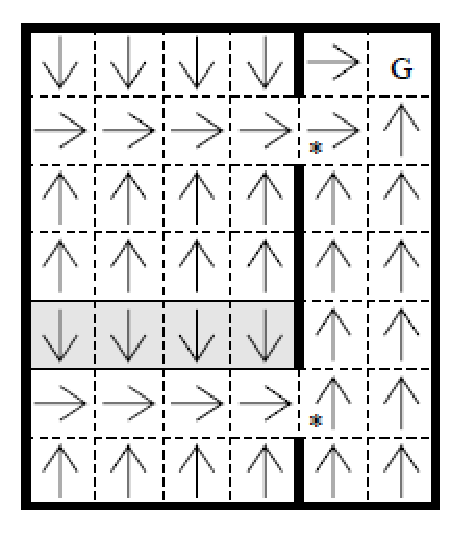
\includegraphics[width=\textwidth] {./figures/Maze.eps}
    \end{minipage}
    \caption{A simple maze problem. The direction of arrow indicates the optimal policy. Figure from \cite{MaxQJ}.}
    \label{fig:Maze}
\end{figure}
\begin{figure}[h]
    \centering
    \begin{minipage}[t]{0.8\linewidth}
        \centering
        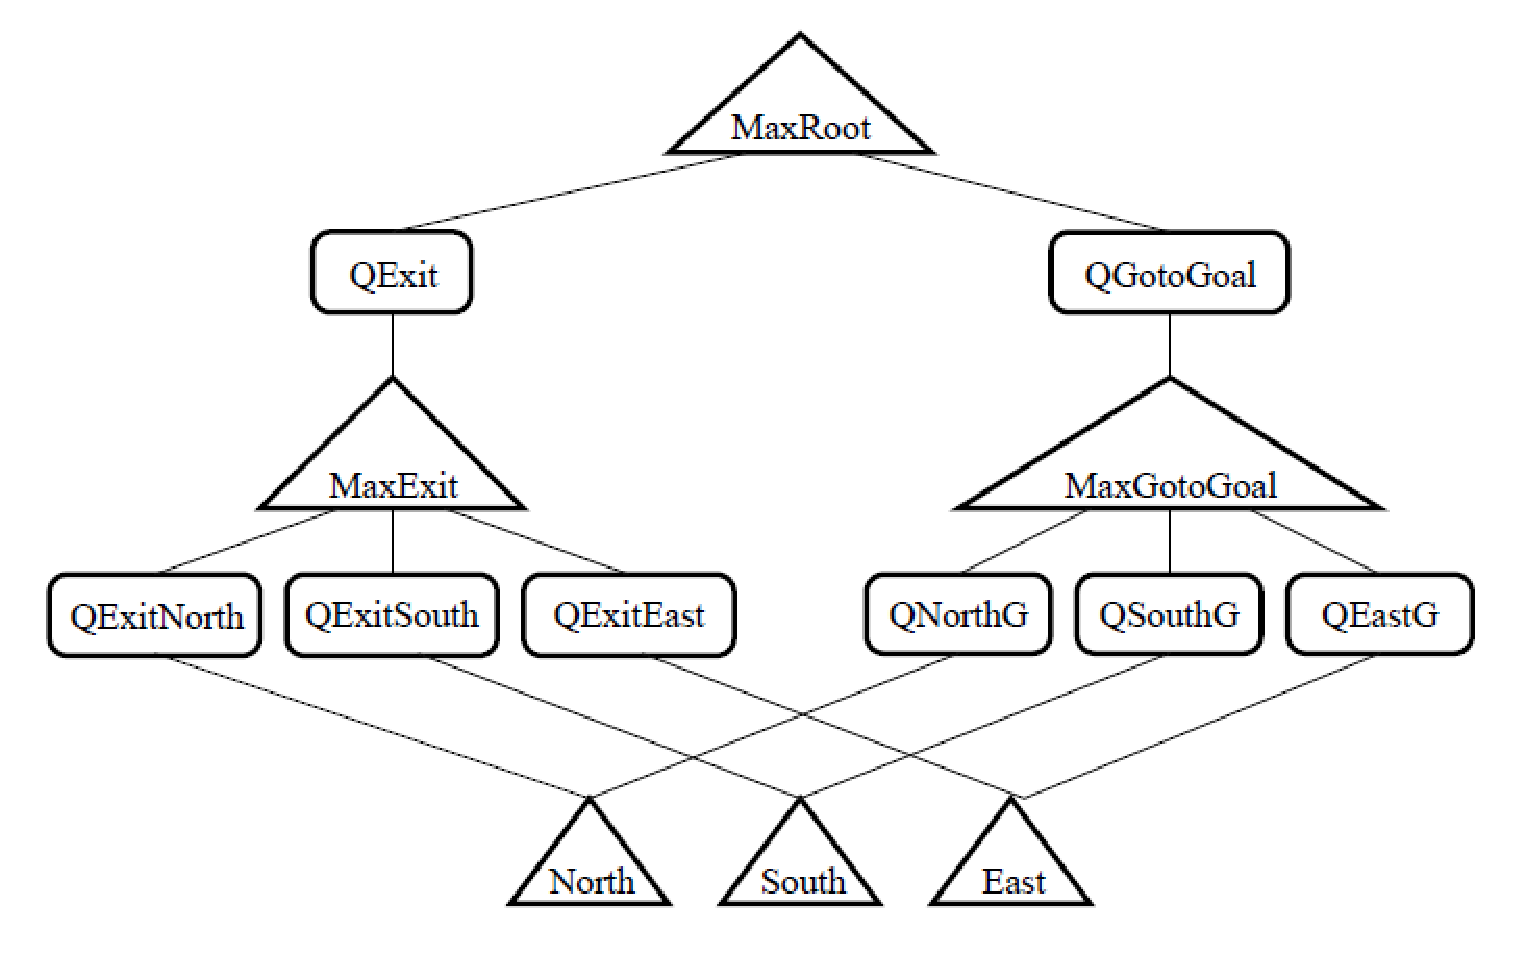
\includegraphics[width=\textwidth] {./figures/MazeH.eps}
    \end{minipage}
    \caption{The hierarchy of maze in Fig. \ref{fig:Maze}. The max nodes are the triangles, and Q nodes are the rectangles. }
    \label{fig:MazeH}
\end{figure}
The hierarchy is shown in Fig. \ref{fig:MazeH}.
"MaxRoot" node corresponds to the root subtask. "MaxGotoExit" corresponds to GotoExit subtask,
and "MaxExit" corresponds to GotoGoal subtask.

In Dietterich's work, all Max nodes are model-free. 
So let us proceed by changing "MaxRoot" node to the model-based one, and let "MaxExit"and "MaxGoal"
to be the regular model-free Max node.
The task for the $i$-th model-based Max node is to compute:
\begin{equation}
    Q^{\pi}(i, s, a) = V^{\pi}(a, s) + C^{\pi}(i, s, a),
\end{equation}
where the completion function $C^{\pi}(i, s, a)$ is the expected cumulative reward after
we complete (composite) action $a$ at state $s$ and before the termination of $i$-th Max node.
$V^{\pi}(a, s)$ is the 
expected cumulative reward when we execute action $a$ at state $s$.
The value $Q^{\pi}(i, s, a)$ is stored in the corresponding Q node.
For example, $Q^{\pi}(MaxRoot, s, GotoExit)$ is stored in "QExit" node.

The node queries its children node to get the value of $V^{\pi}(a, s)$.
It can be computed by:
\begin{equation}
    V^{\pi}(i, s) = \left\{\begin{array}{ll}
                    Q^{\pi}(i, s, \pi_i(s)) & \mbox{if i is composite} \\
                    \sigma_{s'} P(s'|s, i)R(s'|s, i) & \mbox{if $x>y$} \\  
                    \end{array} \right.
    \label{eq:V}
\end{equation}
In our example, to compute $Q^{\pi}(MaxRoot, s, GotoExit)$, "MaxRoot" node would query 
"MaxExit" node to get $V^{\pi}(GotoExit, s)$.

The $C^{\pi}(i, s, a)$ can be computed by the model:
\begin{equation}
    C^{\pi}(i, s, a) = \sum_{s', N}P(s', N|s, \pi(s))\gamma^N[Q^{\pi}(i, s', \pi(s'))].
    \label{eq:C}
\end{equation}

Note that $P(s'|s, \pi(s))$ and $V^{\pi}(a, s)$ are provided by the child Max nodes.

For model-based child Max nodes, $P(s'|s, \pi(s))$ can be computed by equation \ref{eq:multiProb}.

For primitive Max nodes, it can be estimated by:
\begin{equation}
    \tilde{P}(s'|s, a)  = \frac{n(s', s, a)}{n(s, a)},
    \label{eq:countP}
\end{equation}
where $n(s, a)$ is the number of times primitive action $a$ executed 
at state $s$. $n(s', s, a)$ is the number of times primitive action $a$
transitioned the agent from state $s$ to $s'$.

For model-free Max nodes, it can be estimated by \cite{option}:
\begin{equation}
    \tilde{P}(x|s, a) = (1-\alpha)\tilde{P}(x|s, a) + \alpha [ \gamma^N \delta_{s'x}],
    \label{eq:approxP}
\end{equation}
where $s'$ is the observed state after composite action $a$ is executed at state $s$.
$k$ is the number of steps for action $a$ to finish. 
$x$ is the terminal state for the model-free Max node. $\delta_{s'x}=1$ if observed state $s'$
is terminal state $x$ and 0 otherwise.
$\alpha$ is the step-size parameter.
The update of equation \ref{eq:approxP} is conducted after action $a$ terminates at some terminal state,
so we know the exact value of $k$. Note that all of terminal states of the Max node shall be updated after 
action $a$ finished.

We can also use equation \ref{eq:countP} to estimate $\tilde{P}(x|s, a)$, but the policy of the Max node
might change, so equation \ref{eq:approxP} is a better choice.

\section{State Abstraction for model-based Max nodes}
The idea behind model-based approach is to use the sample data to build the model of the environment
and conduct the planning from the model.
The advantage of model-based approaches is that they make more efficient use of the sample data, thus 
it take fewer time to train a model-based RL agent.

The disadvantage is that it needs to compute Q value of all state-action pairs in the current 
planning envelope by Bellman equation (equ. \ref{eq:Q}) until convergence.
Since the number of state-action pairs grows exponentially with the number of features,
it quickly becomes computationally intractable for both time and memory.
For a problem with 9 binary features, the number of states can be $O(2^9)$ and the
number of state-action pairs $(s, a, s')$ can be as large as $2^(9+1+9)=2^19$, which cannot be fit into the
memory of modern computers.

To apply model-based reinforcement learning to large scale problems, 
we need to use some state abstraction technique to reduce the size of planning envelope.

We begin by constructing a projection function $proj(s)$ (it always exists, why?),
which projects state $s$ to an action-invariant space.
That is:
\begin{equation}
    \forall P(s'|s, a) > 0, proj(s') = proj(s)
\end{equation}
It means that the projected state does not change after the execution of 
any actions.
We also needs its dual function $\bar{proj}(s)$ to reconstruct 
the original state $s = \phi(proj(s), \bar{proj}(s))$.

Now we can model $P(s'|s, a)$ by:
\begin{equation}
    P(s'|s, a) = P(\bar{proj}(s')| \bar{proj}(s), proj(s), a)
\end{equation}

Note that we need to query $P(s'|s, a)$ from the child nodes with original representation.
Thus, $\phi(ps, \bar{ps})$ is adopted to compute the original $s'$.  

Although the state abstraction technique above provides us compact state representation, 
it doesn't change the size of the planning envelope. Thus we do not gain any computational
advantage by applying such an abstraction technique.

A key observation of this work is to adopt the approximated projection function which
does not project state $s$ to an action-invariant space.
The size of planning envelope grows exponentially with the number of features.
By assuming 
some features do not change during the execution of actions, we do gain computational advantage by
significantly reducing the size of the planning envelope. 
We lose the optimally with this approximation technique, but it is necessary because we want 
to apply our work beyond toy applications.
Our approach doesn't imply that
some features are completely ignored. The agent still computes the plan according to 
the full state information, but the transition model is simplified to only include the 
relevant information.

\section{Optimality with Biased Model}
The primary contribution of this work is to show that by combining model-based and 
model-free approaches, we can still achieve optimality even when the model is biased.
%Andre and Russell \cite{OptimalQ} extends MaxQ framework to be hierarchical optimal.
%They defined $Q_E(i, s, \pi(s))$ as:
%\begin{equation}
    %Q_E^{\pi}(i, s, \pi(s)) = \Sigma_N \Sigma_{x \in T_i}P(x, N| s, \pi(s)) \gamma^N Q^{\pi}(x, \pi(x)).
    %\label{eq:QE}
%\end{equation}
%$Q_E^{\pi}(i, s, \pi(s))$ is the expected cumulative reward after $i$-th node follows 
%policy $\pi$ at state $s$ and terminates at some point.

\begin{definition}
    Give a hierarchical policy $\pi$ and state $s$, an execution path $E_p^\pi(a_0, s)$ 
    is a set of actions $\{a_0, a_1, \dots, a_{n-1}\}$, where $a_1=\pi_{a_0}(s), a_2=\pi_{a_1}(s), \dots$,
    and $\pi_{a_{n-1}}(s)$ is a primitive action.
\end{definition}
The execution path tells us the order of subtasks which will be invoked for state $s$.


\begin{definition}
    $\mathbb{C}(H) = \{N_1, N_2, \dots, N_k\}$ is a leaf cover of hierarchy $H$ if 
    there exists a composite action $a \in E_p^{\pi}(0, s)$, which belongs to $\mathbb{C}(H)$ for every
    state $s$ and every hierarchical policy $\pi$.
    Furthermore, $\mathbb{C}(H)$ is a total leaf cover if all primitive actions are available for every 
    subtasks $N_i \in \mathbb{C}(H)$.
\end{definition}


%TODO: not all s are defined in Q(i, s, a) (focus on si instead of all i)
%TODO: what if pi_c_bar may change for every step?
%TODO: what if pi_c_bar is not deterministic
%TODO: write down the Q learning algorithm and the model-based one
%TODO: why Q^*(i, s, a) = Q^*(s, a) shows that hierarchical pi is the optimal policy
%TODO: any rigorous property for leaf cover?
%TODO: do I use all assumption for the theorem?
%TODO: the relationship between HORDQ and my approach
%TODO: provide the reason why we need to acceess all primitive action (because of the dumb and never learn planner)
%TODO: show that I can convert any MDP problem to hierarchy one, thus we can always combine approximated model-based approach with HORDQ.

\begin{theorem}
    If $\mathbb{C}(H)$ is a total leaf cover, we have $Q^*(i, s, a) = Q^*(s, a), \forall i \in \mathbb{C}(H)$
\end{theorem}
Proof: Let $\pi_{\bar{\mathbb{C}}}: \mathbb{C}(H) \times S \rightarrow \mathbb{C}(H)$ be the policy to invoke
the next subtask $j = \pi_{\bar{\mathbb{C}}}(i, s)$ which belongs to $\mathbb{C}(H)$. It is determined
by the policy of subtasks which do not belong to $\mathbb{C}(H)$ and terminate predicate $T_i$. Follow Bellman's equation, we have:
\begin{align}
    Q^{\pi}(i, s, a) &= \sum_{s'} P^{\pi}(\pi_{\bar{\mathbb{C}}}(i, s'), s'|i, s, a) [R(s', s, a) + \gamma Q^{\pi}(\pi_{\bar{\mathbb{C}}}(i, s'), s', \pi_i(s'))]\\
    &=\sum_{s'}P^{\pi}(\pi_{\bar{\mathbb{C}}}(i, s')| i, s, a, s') P(s' | i, s, a)  [R(s', s, a) + \gamma Q^{\pi}(\pi_{\bar{\mathbb{C}}}(i, s'), s', \pi_i(s'))]\\
    &\mbox{since $\pi_{\bar{\mathbb{C}}}$ is a deterministic policy}\\
    &=\sum_{s'} P(s' | s, a) [R(s', s, a) + \gamma Q^{\pi}(\pi_{\bar{\mathbb{C}}}(i, s'), s', \pi_i(s'))]
    \label{eq:MaxIrr}
\end{align}

Compare to the Bellman equation of the flat MDP:
\begin{equation}
    Q^{\pi_f}(s, a) = \sum_{s'}P(s'|s, a)[R(s', s, a) + \gamma Q^{\pi_f}(s', \pi_f(s'))].
    \label{eq:bellman}
\end{equation}

The equations \ref{eq:MaxIrr} and \ref{eq:bellman} are identical except for the Q values.
Due to uniqueness of Bellman equation, if $\pi_i(s) = \pi_f(s), \forall s$, we will have $Q^{\pi_f}(s, a) = Q^{\pi_f}(i, s, a)$. 
If $\pi_i(s) = \pi^*_f(s)$, $Q^*(s, a)$ is a solution and also an optimal solution (why?) of equation \ref{eq:MaxIrr}.
Thus we have $Q^*(i, s, a) = Q^*(s, a)$. \textbf{QED.}

%\begin{definition}
    %$\mathbb{C}(H) = \{N_1, N_2, \dots, N_k\}$ is a leaf cover of MaxQ hierarchy $H$ if 
    %we can divide H into several disjoint partitions $P = \{P_1, \dots P_m\}$ after removing all nodes in $\mathbb{C}(H)$.
    %And the root node does not share the partition with any leaf nodes. 
    %$\exists N_i \in \mathbb{C(H)} \suchthat N_i$ is an ancestor of $l$.
%\end{definition}

%\begin{definition}
    %A subtask policy $\pi_i$ is optimal if $\pi_i^{hg*}(s)=\pi_p^*(s) \forall s \in S_i$,
    %where $\pi_p^*(s)$ is the flat optimal policy.
%\end{definition}


%\begin{theorem}
    %If the corresponding subtask policy $\pi_i$ is optimal $\forall N_i \in \mathbb{C}(H)$,
    %the policy $\pi_j$ of the ancestor of $N_i$ is also optimal for all possible $\pi_j$.
%\end{theorem}
%Proof: $\forall N_j$: the ancestor of some node $\in \mathbb{C}(H)$, policy $\pi_j(s)$ would invoke some 
%node $N_i$ and execute its policy $\pi_i^{hg*}(s)$. Since the policy is optimal, $\pi_j^{hg*}(s)=\pi_p^*(s)$.

%\begin{center}
%\begin{tabular}{@{}lp{6cm}@{}}
%\hline
%Algorithm: ExecuteHGPolicy\\
%\hline
%Initialize $\hat{Q_0}$ arbitrarily\\
%$t \leftarrow 0$\\
%Repeat (for each episode)\\
%\ \ \ \ \ \ Initialize $s$\\
%\ \ \ \ \ \ Choose $a$ based on $s$ using policy derived from $\hat{Q_t}$ (e.g., $\epsilon$-greedy method)\\
%\ \ \ \ \ \ Repeat (for each step of episode):\\
%\ \ \ \ \ \ \ \ \ \ \ \ Take action $a$, obtain reward $r$ and next state $s'$ from the environment\\
%\ \ \ \ \ \ \ \ \ \ \ \ Choose $a'$ based on $s'$ using policy derived from $\hat{Q_t}$ (e.g., $\epsilon$-greedy method)\\
%\ \ \ \ \ \ \ \ \ \ \ \ $\hat{q_t} \leftarrow \hat{Q_t}(s, a) + \alpha [r + \gamma \hat{Q_t}(s', a')-\hat{Q_t}(s, a)]$ \\
%\ \ \ \ \ \ \ \ \ \ \ \ Update $\hat{Q_t}$ with $(s, a, \hat{q_t})$ by online L1 regression to produce $\hat{Q_{t+1}}$\\
%\ \ \ \ \ \ \ \ \ \ \ \ $s \leftarrow s'$\\
%\ \ \ \ \ \ \ \ \ \ \ \ $a \leftarrow a'$\\
%\ \ \ \ \ \ \ \ \ \ \ \ $t \leftarrow t+1$\\
%\ \ \ \ \ \ Until $s$ is terminal\\
%\hline  
%\end{tabular}
%\end{center}

%Note that Q function is:
%\begin{align}
    %Q^{\pi}(s, \pi(s)) &= Q^{\pi}(i, s, \pi(s)) + Q_E^{\pi}(i, s, \pi(s))\\
    %&= V^{\pi}(\pi(s), s) + C^{\pi}(i, s, \pi(s)) + Q_E^{\pi}(i, s, \pi(s))
%\end{align}

%Andre and Russell then prove:
%\begin{theorem}
    %If $V^{*}, C^*, Q_E^*$ are solutions to equation \ref{eq:V}, \ref{eq:C},
    %and \ref{eq:QE} for $\pi^*$, then $Q^* = V^{*} + C^* + Q_E^*$ is a solution
    %to the standard Bellman equation.
%\end{theorem}
%\begin{theorem}
    %Decomposed value iteration and policy iteration algorithms derived from equation
    %\ref{eq:V}, \ref{eq:C}, and \ref{eq:QE} converge to $V^{*}, C^*, Q_E^*$, and $\pi^*$.
%\end{theorem}

%However, we need something stronger:
%\begin{theorem}
    %Let $\mathbb\{C\} = \{N_1, N_2, \dots\}$. If 
    %(a) $\forall N_i \in \mathbb{C}$, the descendants of Max node $N_i$ covers all primitive Max nodes
    %and (b) for all path from root node to leaf node must pass at least one of the nodes in $\mathbb{C}$,
    %then the agent has hierarchical optimal policy $\pi^*$ when the policy of node $j \in \{j | j \in subtree(N_i), \forall N_i \in \mathbb{C}\}$.
%\end{theorem}

In Fig. \ref{fig:MazeH}, the agent has an hierarchical optimal policy when "MaxGoal" and "MaxExit"
have the hierarchical optimal policy regardless of the policy of "MaxRoot".

If we let all nodes which are the parent of some primitive Max nodes to have access
to all primitive actions, we can construct $\mathbb{C}$ by including all 
such nodes. Since the optimal policy does not depend on any nodes not in $\mathbb{C}$, 
we can safely replace all such nodes by our approximated model-based nodes.

For example, if we replace "MaxRoot" with approximated model-based nodes,
the policy is still optimal. 

The problem of this hierarchical optimal approach is that policy $\pi_i$ of $i$-th
node is determined by the expected cumulative reward, not by the expected pseudo reward as
MaxQ. Due to the lack of pseudo reward, each subtask $M_i$ lacks the motivation to 
pursue the goal state defined by the hierarchy, thus it makes the hierarchical 
design useless. 
It is necessary to add some pseudo reward to encourage each subtask to pursue 
the goal. Nevertheless, it should be done carefully, otherwise we will lose
the optimality.

Here we show a way to add the pseudo reward without violating the hierarchical 
optimal constraint:
\begin{theorem}
    Let $x$ be some terminal state of subtask $M_i$, $R(x)$ be the reward
    when the agent arrives state $x$, $\tilde{R}(x) = R(x) - r$ be the pseudo reward
    and $r$ be the penalty term.
    If $P(x| s, \pi_i^*(s)) = 0$, we have $Q^*(i, s, \pi^*(s)) = \tilde{Q}^*(s, \tilde{\pi}(s))$.
\end{theorem}

The above theorem says that the optimal policy does not change 
if some penalty is applied at some terminal states which are not part of the optimal path.


%We need the penalty for the hierarchy to work. 
%Since we do not usually know what the optimal policy is, we may add penalty term in 
%wrong states and lose the optimality. But we do not always require 


The idea of our work is to use the approximated model-based node to 
compute the plan for the agent, and let the hierarchical optimal model-free node
to execute the plan. If everything works as the plan, the agent would converge to the optimal
policy in a short time. If not (following the plan is worse than the penalty term),
the model-free node will take control and find the optimal policy on its own.

The penalty term serves as a mechanism to enforce the subtask to follow the hierarchy.
The subtask will strictly follow the subgoal defined by the hierarchy if the penalty term is large.
On the other hand, if the penalty term is small, the subtask is more likely to go rouge and try to 
solve the whole problem on its own. Here we have a engineering decision: if we trust our hierarchy design, 
we should increase the penalty term to let the agent find the optimal policy as fast as it can; 
if not, a low penalty term allows the agent to find the optimal policy when the hierarchy doesn't work.

%show that the exact condition (the certain hierarchy) for the conjecture to work (iff)
%Show that use decision tree to predict next state is bad (because the planning envelope is too big)
%if a coin is 20 steps away, and there is a random walk monster, the planning envelope is 2^20
%use this to motivate why we need to assume something does not change
%Also show that the drawback of peter stone's work on approximated model based approach

%\section{Temporal Difference Learning}

%The RL agent estimates the $Q_{E}$ by SARSA algorithm -- after the RL agent takes the action $a$
%and observes next state $s'$, reward $r$ and next action $a'$, the $Q_{E}$ is updated by:
%\begin{equation}
    %Q_{E}^{g, t}(s, a) \leftarrow  Q_{E}^{g, t}(s, a) + \alpha [r + \gamma Q_{E}^{g, t-1}(s', a') - Q_{E}^{g, t}(s, a)]
%\end{equation}

%The RL agent estimates the probability to achieve the goal by the same equation:
%\begin{equation}
    %P^{g, t}(s, a) \leftarrow  P^{g, t}(s, a) + \alpha [\delta + \gamma P^{g, t-1}(s', a') - P^{g, t}(s, a)]
%\end{equation}


%\section{The Problem of Unsafe State Abstraction}
%1. introduce poison problem
%2. why unsafe abstraction cannot do
%3. how to relief the burden by incorporation of model free node
%4. Why relief (what it cannot do)
%5. Motivating the hierarchical node (no pseudo reward)
%6. Achieve optimality with biased model
%7, The problem of hierarchical optimal approach
%8. Show that how the degree of hierary penalty changes the behavior of the agent (by the experiment)

%\section{Hierarchical Optimality}
%To compensate the incapability to predict the movement of the monsters in the long run, 
%we exploits the model-free approach to handle the dynamic of the environment in the short period.
%The choice

%Besides, the model-free layer still operates with the full observation of the state. 
%If we put more features into the model-based layer, we would get a more precise plan at the cost
%of more samples required to estimate the model parameter and more time spent on computing the plan.
%Therefore, the number of features included in the model-based layer depends on the available 
%computation resources.
%The objective of our work is not to show how to find the optimal arrangement of features, but to indicate
%that there is a trade-off between model-based and model-free approaches.
%By adjusting the arrangement of features, we can maximize the performance of the agent without exceeding
%the capacity of available computational resources.

%\section{Estimation of the transition probability}

%Each max node (except the top one) needs to compute the state transition probability
%from the given state $s$ to some terminal state $x$.
%It can be done by querying the transition probability from the child layers.
%Same for the reward.

%Each model-free layer with a parent model-based layer also needs to compute the transition probability.
%Since the child layers of model-free layer do not provide such information, the model-free layer
%needs to estimate the probability based on its current policy.

%TODO: the grid world example--> assuming monster does not move is correct
%TODO: show that approximation is necessary--> the planning envelope is exponentially huge wrt the number of monsters




%This stochastic natural of the game makes it natural to formulate the problem as a stochastic shortest path
%problem. A stochastic shortest-path (SSP) problem is a MDP problem with a absorbing goal state and positive costs.
%A solution of a SSP problem is a policy from the initial state to the goal state with minimum expected cost.

%A work by Zucker et al. \cite{Planner} introduced a two-level approach to solve a maze problem.
%The planner uses the shortest path algorithm to find a path from the current state to the goal state.
%The cost of each step is estimated by Q value, which is computed by the SARSA algorithm.

%A issue occurred when we want to apply this approach to general MDP problems: we do not know the 
%goal state. The objective of MDP is to find a sequence of actions which can maximize the overall 
%rewards. There are no clearly defined "goal" for the MDP problems.

%A possible way to adopt the planning technique to the MDP problems is to choose a sequence 
%of goals which can maximize the overall rewards. The goal can be chosen to be the state
%with the highest expected reward. To achieve this, an agent needs to learn 
%the probability to move from one state to another, and the reward to be received
%from each state. 

%The approach is two fold. In the beginning, the planner selects a path from the current 
%state to the goal state with the highest expected reward. The path consists of several
%nodes, which are considered as the subgoals of the plan. The RL agent finds the subgoal 
%right after the current state, and chooses a sequence of actions which can lead the agent
%to the subgoal. The result can be either success or failure, and the probability of the successful
%rate of a plan would be updated accordingly. The planner then use the updated information to 
%compute a new path.

%%\section{The task hierarchy of eat-food-and-avoid-monster game}
%%\section{Training the RL agent}
%The training is done in $5 \times 5$ with one food and one monster.
%A goal is assigned to the agent at the beginning of the episode. 
%The goal is the desired next position of the agent.
%%The goal is the position difference of 
%%the current position and the next position. It can be either $(0, 1), (0, -1), 
%%(1, 0) or (-1, 0)$.
%The action of the agent terminates after 1 step regardless if the agent achieves the goal 
%or not. The task of the RL agent is to find an optimal policy to achieve the goal. 
%Although the optimal policy is obviously corresponding to the four primitive actions (north, south, west or east) 
%, the agent doesn't have any prior knowledge of it. Moreover, the agent should not always comply to the indication of the goal.
%If the goal asks the agent to go north but there is a monster at north of the agent, it is unwise to go north to achieve the goal.

%To construct a RL agent which may follow the instruction of the planner when possible, 
%we give the reward of the RL agent $+20$ when it achieves the goal and $0$ otherwise.
%If the agent gets into a monster, it receives $-30$ reward as usual.

%The planner makes the plan based on the state transition probability and the corresponding reward for each transition.
%The RL agent needs to provides such an information to the planner (note that the state transition probability and the reward
%depends on the current RL agent policy).
%The information must be learned as well. 
%The reward given by the planner (like the reward for achieving the goal) is called internal reward.
%The internal reward is constructed to get the desired behavior of the RL agent.

%The reward given by the game itself is called external reward.  It is what the
%planner tries to maximize. The expected external reward for the agent to move
%from current state $s$ to the goal state $g$ within $t$ steps is:

%\begin{equation}
    %R_{E}(g, s, t) = Q_{E}^{g, t}(s, \pi(s)), 
%\end{equation}
%where $\pi$ is the policy of the RL agent which directs it agent to go to the goal state within $t$ steps.
%$\pi(s)$ is one of the primitive actions.
%$Q_{E}$ is the expected external reward function for the agent to get at state $s$ if 
%the RL agent takes action $\pi(s)$.

%The RL agent estimates the $Q_{E}$ by SARSA algorithm -- after the RL agent takes the action $a$
%and observes next state $s'$, reward $r$ and next action $a'$, the $Q_{E}$ is updated by:
%\begin{equation}
    %Q_{E}^{g, t}(s, a) \leftarrow  Q_{E}^{g, t}(s, a) + \alpha [r + \gamma Q_{E}^{g, t-1}(s', a') - Q_{E}^{g, t}(s, a)]
%\end{equation}

%The RL agent estimates the probability to achieve the goal by the same equation:
%\begin{equation}
    %P^{g, t}(s, a) \leftarrow  P^{g, t}(s, a) + \alpha [\delta + \gamma P^{g, t-1}(s', a') - P^{g, t}(s, a)]
%\end{equation}

%$\delta$ is 1 when the RL agent achieves the goal state (if $s'$ is the goal state) and 0 otherwise.

%The policy $\pi(s)$ of the RL agent is determined by the expected internal reward function $Q_{I}$.
%\begin{equation}
    %\pi(s) = argmax_a Q_{I}^{g, t}(s, a), 
%\end{equation}
%Similarly, $Q_{I}$ can be estimated by SARSA algorithm.

%\begin{figure}[h]
    %\centering
    %\begin{minipage}[t]{0.9\linewidth}
        %\centering
        %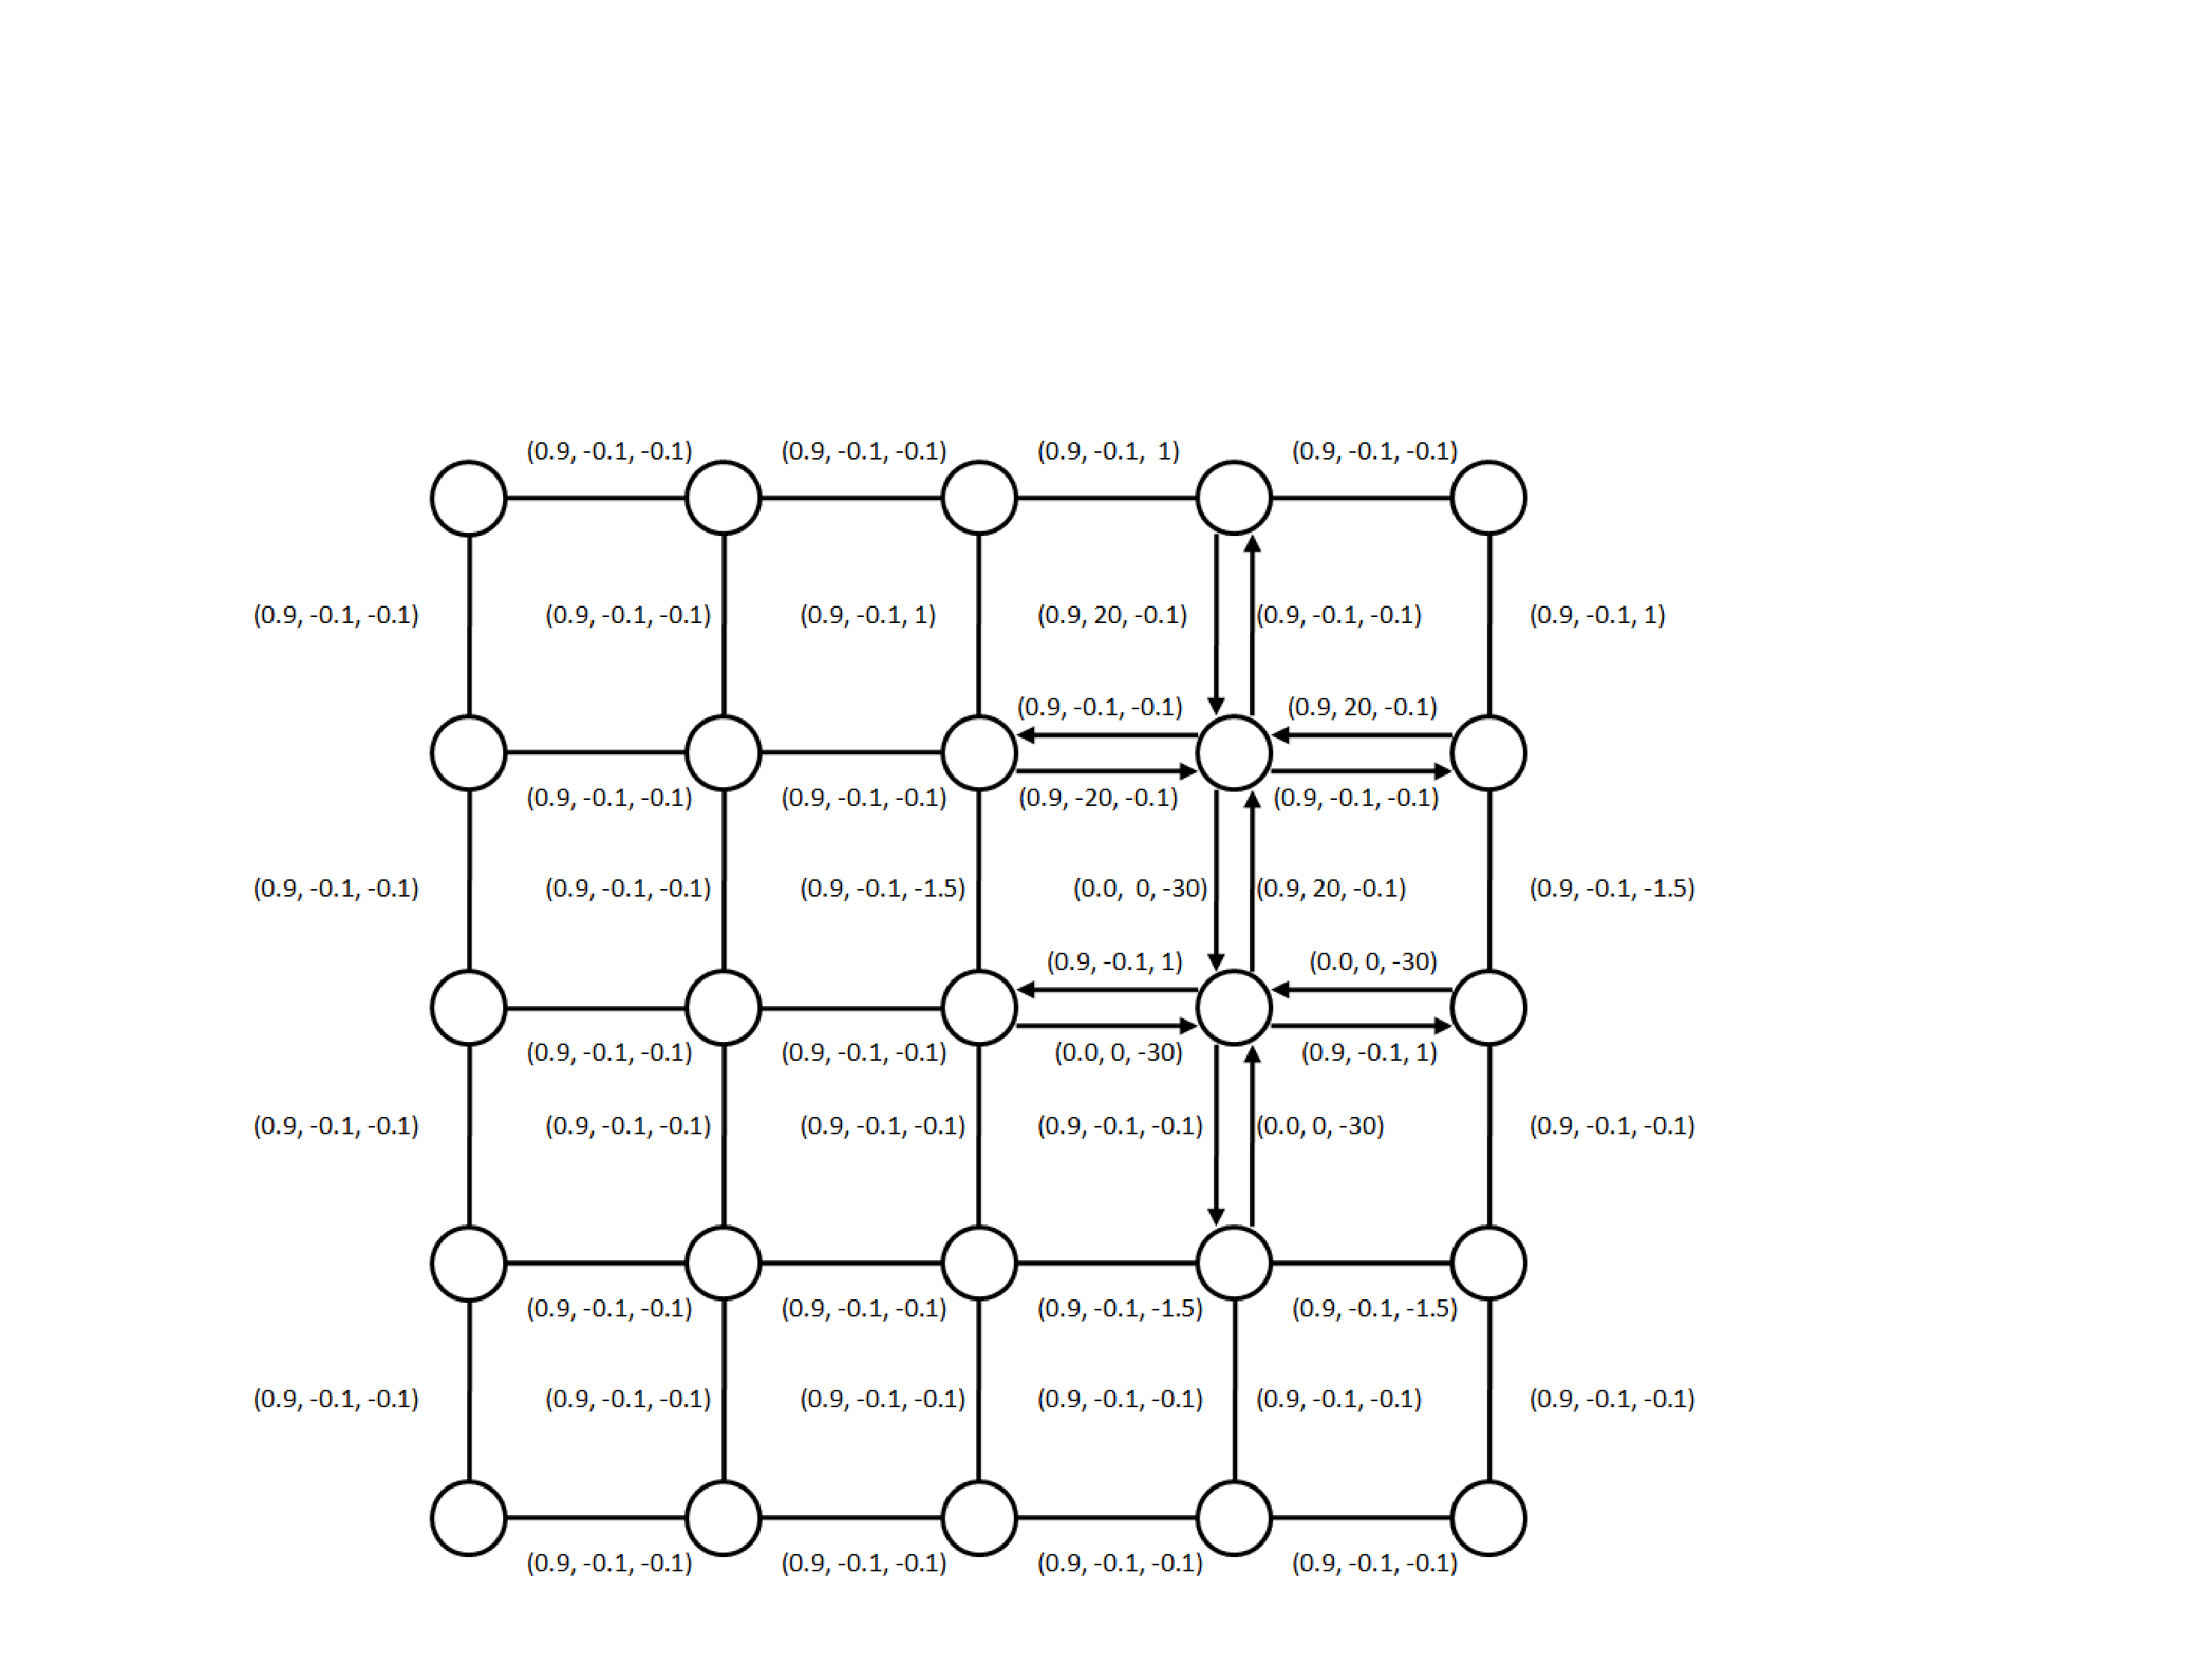
\includegraphics[width=\textwidth] {./figures/PlanGraph.eps}
    %\end{minipage}
    %\caption{The transition probability and reward for the game in Fig. \ref{fig:MonsterPlan}}
    %\label{fig:PlanGraph}
%\end{figure}

%To construct a plan, the planner uses shortest-path algorithm to find a path with maximum expected reward.
%For example, the plan in Fig. \ref{fig:MonsterPlan} corresponding to the expected reward of 
%$18*0.9^5$ with the estimated transition probability and)reward shown in Fig. \ref{fig:PlanGraph}.
%In general, the expected reward of the plan $p = (s_1, s_2, \dots, s_n)$ can be computed by: 
%\begin{equation}
    %R_P(p) = R_E(s_2, s_1, t) + R_E(s_3, s_2, t)P^{s_2, t}(s1, \pi(s1)) + \dots + R_E(s_n, s_{n-1}, t)P^{s_n, t}(s_{n-1}, \pi(s_{n-1})) \dots P^{s_2, t}(s1, \pi(s1))
%\end{equation}



\endinput
%Most of the previous work on RL focus on model-free approaches for several reasons. 
%The most 
%Within a planning agent, there are at least two roles for real experience: it
%can be used to improve the model (to make it more accurately match the real
%environment) and it can be used to directly improve the value function and
%policy using the kinds of reinforcement learning methods we have discussed in
%previous chapters. The former we call model-learning, and the latter we call
%direct reinforcement learning (direct RL). The possible relationships between
%experience, model, values, and policy are summarized in Figure  9.2. Each arrow
%shows a relationship of influence and presumed improvement. Note how experience
%can improve value and policy functions either directly or indirectly via the
%model. It is the latter, which is sometimes called indirect reinforcement
%learning, that is involved in planning. 

%The second branch is model-based RL, which directly estimates
%a model of the environment and then plans with
%this model. Early work demonstrated that summarizing an
%agent’s experience into a model could be an efficient way
%to reuse data (Moore & Atkeson, 1993), and later work utilized
%the uncertainty in an agent’s model to guide exploration,
%yielding the first (probabilistic) finite bounds on the amount of data required
%to learn near-optimal behaviors in the general case (Kearns & Singh, 1998;
%Kakade, 2003).


%motivation: play a randomly generate maze to adapt to
%adapt to noval situation

%weakness-> an adversary to block the path forever
%no knowledge (coin won't disappear-->need hack to do it, moster won't move)
%comparison to the previous work->HRL,


%model based-> state space is too large. good to train with
%few examples (10 sec training)
%model free-> cannot handle randomly generated maze -> failed to adapt to noval situation. can handle large space (linear SARSA)
%Experiment: comparison with flat model based approach and hierarchical model based approach with approximation

%combine both-> use model based on top level to reduce
%the state space, and model free on bottom to 
%deal with randomized noisy world for short term reward

%build multilevel of hierachy on features
%label each room with a number 1, 2, 3
%the coordinate of wrt the room
%(1, (25, 30))
%move from room 1 to room 2
%top level
%action (1->2)
%second level
%assume (1, (25, 30)) -> (2, (0, 0))
%action ((25, 30) -> (0, 0)) goal (-25, -30) in single step

%need to build time model of the full state
%P(s->s'|x, t) the propability to move from state s to s'
%after t steps of the observation of full state x

%power coms from trasition model (model the shortest path), not shortest path
%you can use model-based approach on this

%fickle passenger of MaxQ
%coarseness on time and space scale

%-->you can work on continus varible now, no more grid world

%1. Assumption on the state difference (if it is not true --> like the agent in a world boundary or the health is 100 and cannot be imporve
  %since the state is outside the known state boundary, the planner whon't plan for it. but the local planner may still direct the agent
  %to go outside the world boundary, which may be a problem)
%2. Application to the hierachical RL
%3. Limitation: unachievable state (a coin surrounded by many monsters)
%4. Can inference in a very small world, not need to do 64 by 64
%Sometimes we need a plan. The greedy approach of reinforcement learning does not always work. 
%RL techniques have several limitations:
%1. It's difficult for to transfer the value function from a small world to a large one. If the agent has
%the experience only in a small world like 4 \times 4 grid, it cannot act well in 64 \times 64 grid
%because it does not know the correct action in regard to an object 63 grid away.

%2. It takes a long time to train the agent to be good enough. The greedy 

%3. The approximation only good in a small range. We need a plan for long term action.
%The noval state (the state in current game which has not been experienced) may 

%4. Impossible task to maze problems: RL require that optimal agent to find the optimal solution for a maze when all the features
%are input to the agent. Which is unlikely to work.(impractical when the maze is large)(unable to transfer
%the knowledge from previous maze experience to the current one) A practical solver shall invovle planning through 
%the possible route and find the one which can lead to the exist.
%All the work requires the agent to repeat play the same maze (assuming traps) until it finds the optimal solution.
%What if the maze changes every time?

%1. Is it guarranteed convergence? Yes, if we choose the goal next to the current state which leads to highest Q value. 
%It is the same as SARSA.
%2. How to choose the goal to guarrante convergence to optimal policy?

%Good to work on the problem with a long term reinforcement (feedback) like a maze.
%Bad to work with a problem with dynamic envirment (everything changes with or without agents actions)
%Bad when the consequence of an action is delayed for many steps. (poison)

%Q: prove that RL cannot solve maze problem
%Ability to transfer the knowledge from one maze to another
%compare the HRL in key-finding problem
%compare to the model-based RL





%application: the key-room problem--> each room lock a key, one room has a treasure, the agent needs to go through 
%a maze to collect the keys for each door and get the treasure

%Stochastic Shortest-Path Problems
%A Stochastic Shortest-Path problem is an mdp prob-
%lem in which the state space S = f1; : : : ; n; tg is such
%that t is a goal (target) state that is absorbing (i.e.,
%p(t; u; t) = 1 and g(t; u) = 0 for all u 2 U(t)), and the
%discount factor ® = 1. In this case, the existence of
%optimal policies (and optimal stationary policies) is a
%major mathematical problem. However, the existence
%is guarantee under the following reasonable conditions:
%(A1) There exists a policy that achieves the goal with
%probability 1 from any starting state.
%(A2) All costs are positive.
%The ¯rst assumption just expresses the fact that the
%problem admits a well-behaved solution. Such policies
%are known as proper policies. The second assumption,
%in the other hand, guarantees that all improper policies
%incurs in in¯nite cost for at least one state. Thus, both
%assumptions preclude cases where the optimal solution
%might \wander" around without never getting to the
%goal. For example, a problem having a zero-cost cycle
%(in state space) violates the second assumption.
%As mentioned in the Introduction, often we are only
%interested in knowing how to go from a ¯xed initial
%state, say 1, to the goal state. The optimal solution in
%this case is an partial optimal stationary policy ¹ such
%that ¹(i) = ¹¤(i) for all states i that are reachable
%from 1 when using the optimal policy ¹¤; the so-called
%relevant states when starting from 1.1
%Finding a partial optimal policy can be consider-
%ably simpler, the extreme case when the set of relevant
%states is ¯nite and the complete state space is in¯nite.
%Thus, the question of how to ¯nd partial optimal poli-
%cies is of great relevance. One algorithm for that is
%Real-Time Dynamic Programming.

%There are two ways for a RL agent to use its sample data. It can use the sample data to update the 
%value function and improve its policy. It is called model-free (or direct) reinforcement learning. 
%Another approach is to use the sample data to estimate parameters for the model of the environment and compute the value function
%from the model. It is called model-based (indirect) reinforcement learning.

%The advantage of model-based approaches is that they make more efficient use of the sample data, thus 
%it take fewer time to train a model-based RL agent. Other the other hand, model-free approaches do not assume 
%a prior model, so it would not be affected by the bias of the model design. Besides, the existence of 
%good linear approximation algorithms, such as linear SARSA, makes it possible for model-free approaches to
%handle large scale problems.

%Model-based approaches needs to enumerate through all possible states to compute the value function. 
%But the number of states grows exponentially with the number of features, 
%and it quickly becomes intractable if the number features grows large.

%The main idea of this work is to combine the model-free, model-based and hierarchical reinforcement learning.
%For the lower level of hierarchy, we adopt the model-free approach to handle the complete and possibly large state space.
%On the top level of hierarchy, we use the model-based to plan on a coarser level, which contains only small number of states.
%This approach allows the agent to plan on the higher level and make efficient use of the sample data. On the lower level,
%the agent uses model-free approaches with linear approximation to handle the complete state space.

%The prior works on hierarchical reinforcement learning (HRL) can be divided into two categories: model-free and model-based approaches. 
%The model-free approaches include HAMQ \cite{HAMQ}, MAXQ \cite{MAXQ}, SMDP and options framework \cite{option}
%For model-based approaches, Seri et al. \cite{HLearning} proposed a model-based HRL in average reward setting.
%Diuk et al. \cite{Diuk} adopted model-based HRL to deterministic domain. Jong and Stone \cite{RMaxQ} combined 
%R-MAXQ and MAXQ to achieve efficient model-based exploration and the action abstraction of MAXQ.

%TODO: show that model based state difference can learn randomly generated maze with very limited steps (only four touches of the wall)
%TODO: use a poison example to show the limit of pure approximated model-based approach and the motivation
%of use hierarchical optimal policy for pseudo reward and recursive optimal policy for real reward. It can be shown that
%it will converge to optimal policy if the true goal state of the game is included as a subgoal(
%the worst case is the child node finish the game by itself)
